\documentclass[letterpaper,12pt]{article}
\usepackage{array}
\usepackage{threeparttable}
\usepackage{geometry}
\geometry{letterpaper,tmargin=1in,bmargin=1in,lmargin=1.25in,rmargin=1.25in}
\usepackage{fancyhdr,lastpage}
\pagestyle{fancy}
\lhead{}
\chead{}
\rhead{}
\lfoot{}
\cfoot{}
\rfoot{\footnotesize\textsl{Page \thepage\ of \pageref{LastPage}}}
\renewcommand\headrulewidth{0pt}
\renewcommand\footrulewidth{0pt}
\usepackage[format=hang,font=normalsize,labelfont=bf]{caption}
\usepackage{listings}
\lstset{frame=single,
  language=Python,
  showstringspaces=false,
  columns=flexible,
  basicstyle={\small\ttfamily},
  numbers=none,
  breaklines=true,
  breakatwhitespace=true
  tabsize=3
}
\usepackage{amsmath}
\usepackage{amssymb}
\usepackage{amsthm}
\usepackage{harvard}
\usepackage{setspace}
\usepackage{float,color}
\usepackage[pdftex]{graphicx}
\usepackage{hyperref}
\hypersetup{colorlinks,linkcolor=red,urlcolor=blue}
\theoremstyle{definition}
\newtheorem{theorem}{Theorem}
\newtheorem{acknowledgement}[theorem]{Acknowledgement}
\newtheorem{algorithm}[theorem]{Algorithm}
\newtheorem{axiom}[theorem]{Axiom}
\newtheorem{case}[theorem]{Case}
\newtheorem{claim}[theorem]{Claim}
\newtheorem{conclusion}[theorem]{Conclusion}
\newtheorem{condition}[theorem]{Condition}
\newtheorem{conjecture}[theorem]{Conjecture}
\newtheorem{corollary}[theorem]{Corollary}
\newtheorem{criterion}[theorem]{Criterion}
\newtheorem{definition}[theorem]{Definition}
\newtheorem{derivation}{Derivation} % Number derivations on their own
\newtheorem{example}[theorem]{Example}
\newtheorem{exercise}[theorem]{Exercise}
\newtheorem{lemma}[theorem]{Lemma}
\newtheorem{notation}[theorem]{Notation}
\newtheorem{problem}[theorem]{Problem}
\newtheorem{proposition}{Proposition} % Number propositions on their own
\newtheorem{remark}[theorem]{Remark}
\newtheorem{solution}[theorem]{Solution}
\newtheorem{summary}[theorem]{Summary}
%\numberwithin{equation}{section}
\bibliographystyle{aer}
\newcommand\ve{\varepsilon}
\newcommand\boldline{\arrayrulewidth{1pt}\hline}


\begin{document}

\begin{flushleft}
  \textbf{\large{Problem Set \#2}} \\
  MACS 40200, Dr. Evans \\
  Bobae Kang
\end{flushleft}

\vspace{5mm}

\noindent\textbf{1. Health claim amounts and the GB family of distributions}
\par
\noindent(a) Calculate and report the mean, median, maximum, minimum, and standard deviation of monthly health expenditures for these data. Plot two histograms of the data in which the y-axis gives the percent of observations in the particular bin of health expenditures and the x-axis gives the value of monthly health expenditures.
\par\bigskip

The descriptive statistics of the data are as follows:
\begin{table}[h!]
 \centering
 \caption{The descriptive statistics of the data }
 \begin{tabular}{|c | c |} 
  \hline
  Mean &  720.277975327\\ 
  Median &  172.21\\ 
  Maximum &  227967.25\\ 
  Minimum &  0.01\\ 
  Standard Deviation &  3972.66375639\\ 
  \hline
  \end{tabular}
\end{table}
\par

The following two graphs are the hisograms of the data 
\begin{figure}[H]\centering\captionsetup{width=4.0in}
   \caption{\textbf{A histogram of the health claims from a fictitious sample households}}
   \fbox{\resizebox{4.0in}{3.0in}{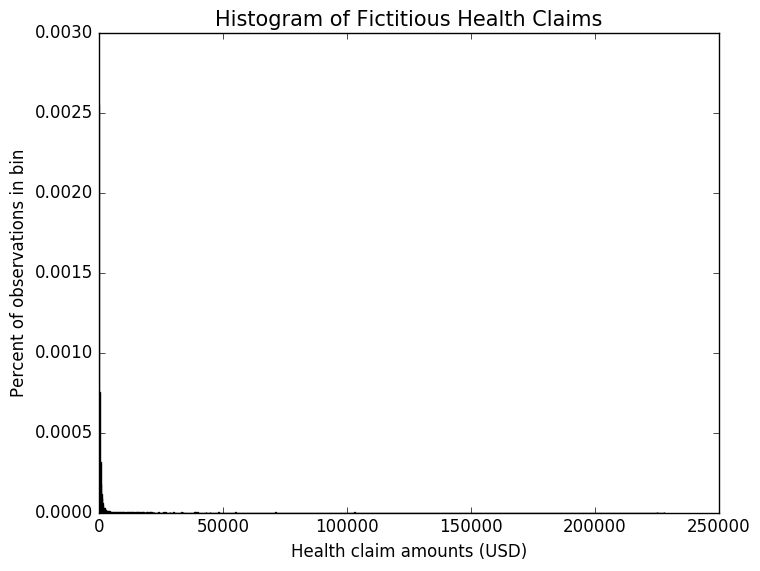
\includegraphics{./images/fig_1a_1.png}}}
\end{figure}
\par
\begin{figure}[H]\centering\captionsetup{width=4.0in}
   \caption{\textbf{A histogram of the health claims from a fictitious sample households, $\leq \$800$}}
  \fbox{\resizebox{4.0in}{3.0in}{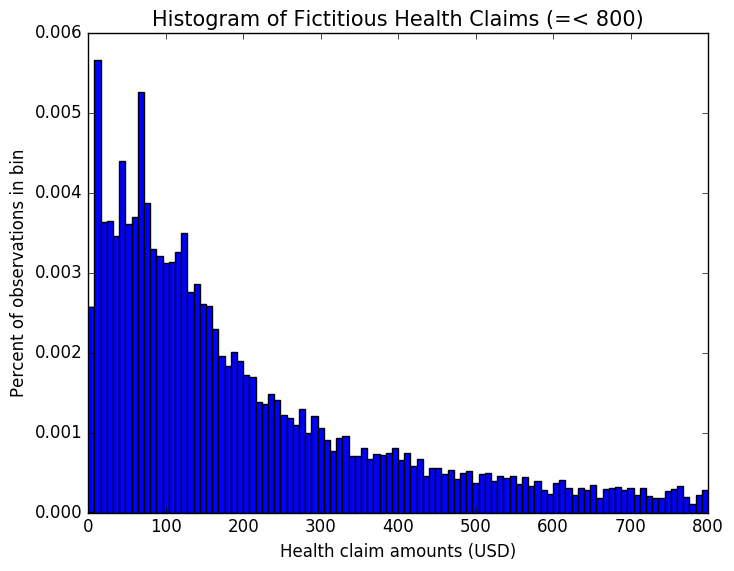
\includegraphics{./images/fig_1a_2.png}}}
\end{figure}
\par\bigskip

\noindent(b) Using MLE, fit the gamma distribution to the individual observation data. Report your estimated values for parameters, as well as the value of the maximized log likelihood function. Plot the second histogram from part (a) overlayed with a line representing the implied histogram from your estimated gamma distribution.
\par\bigskip

\begin{table}[h!]
 \centering
 \caption{MLE results using the gamma distribution}
 \begin{tabular}{|c | c |} 
  \hline
  $\hat{\alpha}_{MLE}$ & 0.221755308612 \\ 
  $\hat{\beta}_{MLE}$ & 21911.0646993\\
  Log-likelihood & -82076.4516057\\
  \hline
  \end{tabular}
\end{table}
\par
VCV =  [[  4.37717820e-06   9.32885080e-05]\par
 [  9.32885080e-05   1.00000060e+00]]
\par

\begin{figure}[H]\centering\captionsetup{width=4.0in}
  \caption{\textbf{Fitting the gamma distribution using MLE, $\leq \$800$}}
  \fbox{\resizebox{4.0in}{3.0in}{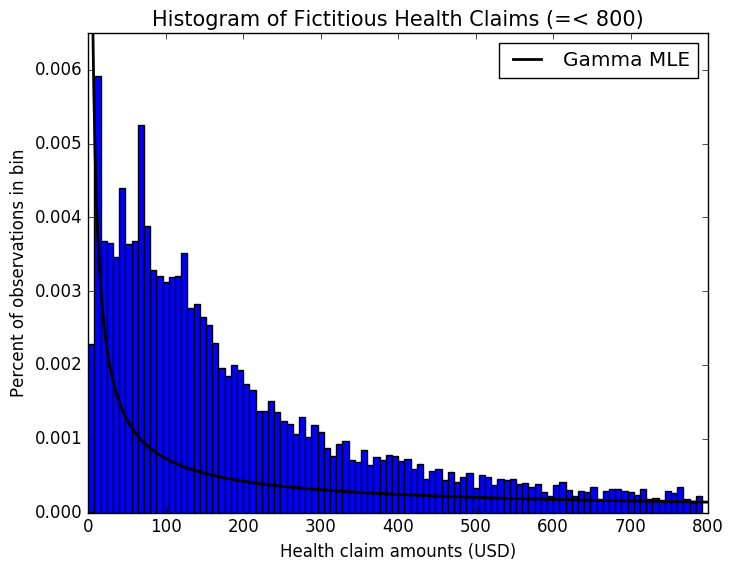
\includegraphics{./images/fig_1b.png}}}
\end{figure}
\par\bigskip

\noindent(c) Using MLE, fit the generalized gamma distribution to the individual observation data. Use your estimates for $\alpha$ and $\beta$ from part (b), as well as m = 1, as your initial guess. Report your estimated values for parameters, as well as the value of the maximized log likelihood function. Plot the second histogram from part (a) overlayed with a line representing the implied histogram from your estimated generalized gamma distribution.
\par\bigskip

\begin{table}[h!]
 \centering
 \caption{MLE results using the generalized gamma distribution}
 \begin{tabular}{|c | c |} 
  \hline
  $\hat{\alpha}_{MLE}$ & 0.222276613384 \\ 
  $\hat{\beta}_{MLE}$ & 21911.0644724 \\
  $\hat{m}_{MLE}$ & 0.997648454581\\
  Log-likelihood & -82076.446472\\
  \hline
  \end{tabular}
\end{table}
\par
VCV =  [[  3.08655089e-05  -1.52641448e-05  -1.51784572e-04]\par
 [ -1.52641448e-05   1.00903661e+00   5.29737394e-03]\par
 [ -1.51784572e-04   5.29737394e-03   4.58901429e-02]]
\par

\begin{figure}[H]\centering\captionsetup{width=4.0in}
  \caption{\textbf{Fitting the generalized gamma distribution using MLE, $\leq \$800$}}
  \fbox{\resizebox{4.0in}{3.0in}{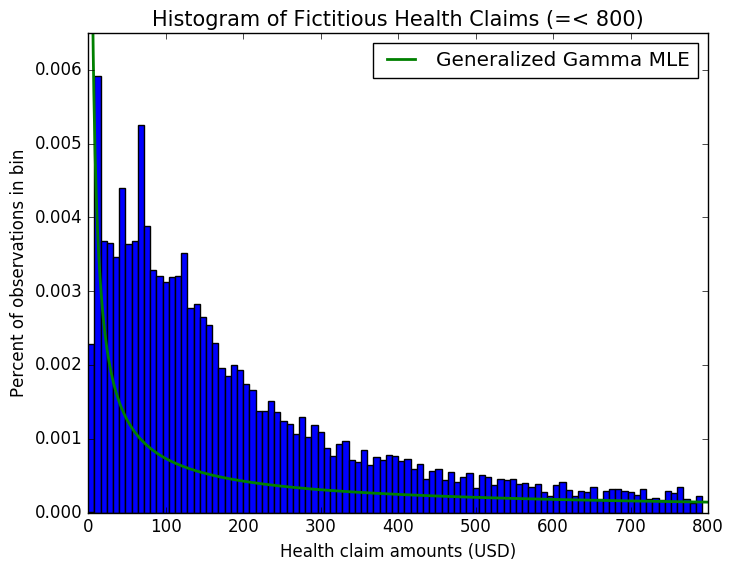
\includegraphics{./images/fig_1c.png}}}
\end{figure}
\par\bigskip

\noindent(d) Using MLE, fit the generalized beta 2 distribution to the individual observation data. Use your estimates for $\alpha$, $\beta$ and $m$ from part (c), as well as $q = 10,000$, as your initial guess. Report your estimated values for parameters, as well as the value of the maximized log likelihood function. Plot the second histogram from part (a) overlayed with a line representing
the implied histogram from your estimated generalized beta 2 distribution.
\par\bigskip

\begin{table}[h!]
 \centering
 \caption{MLE results using the generalized gamma distribution}
 \begin{tabular}{|c | c |} 
  \hline
  $\hat{a}_{MLE}$ & 0.699528434728 \\ 
  $\hat{b}_{MLE}$ & 223919455.619 \\
  $\hat{p}_{MLE}$ & 0.995695905023 \\
  $\hat{q}_{MLE}$ & 10001.8955911\\
  Log-likelihood & -76461.5898932\\
  \hline
  \end{tabular}
\end{table}
\par
VCV =  [[  8.47578124e-03   0.00000000e+00  -1.03428896e-01  -1.15211264e+00]\par
 [  0.00000000e+00   1.00000000e+00   0.00000000e+00   0.00000000e+00]\par
 [ -1.03428896e-01   0.00000000e+00   1.26223521e+00   1.40607231e+01]\par
 [ -1.15211264e+00   0.00000000e+00   1.40607231e+01   1.56664117e+02]]
 \par

\begin{figure}[H]\centering\captionsetup{width=4.0in}
  \caption{\textbf{Fitting the generalized beta 2 distribution using MLE, $\leq \$800$}}
  \fbox{\resizebox{4.0in}{3.0in}{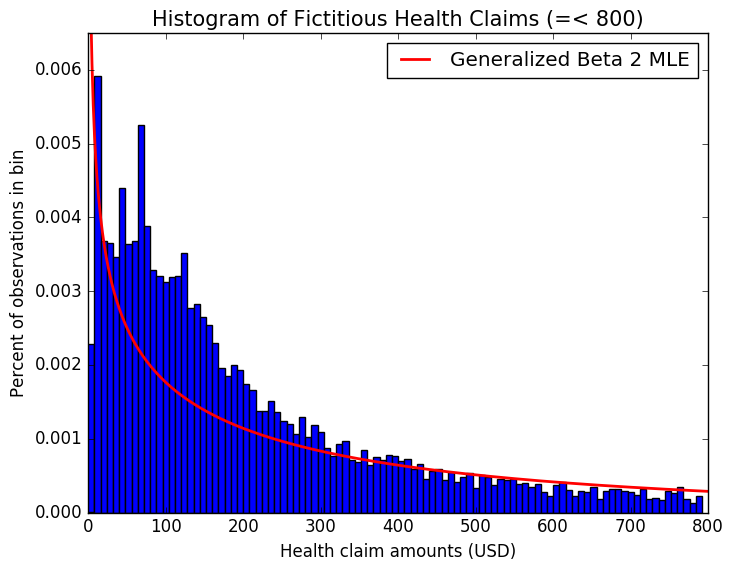
\includegraphics{./images/fig_1d.png}}}
\end{figure}
\par\bigskip

\noindent(e) Perform a likelihood ratio test for each of the estimated in parts (b) and (c), respectively, against the GB2 specication in part (d). Report the chi-square(4) values from the likelihood ratio test for the estimated GA and the estimate GG.
\par\bigskip
$\chi^2$ of $H_{0}: ga = gb2$ with 4 degrees of freedom p-value =  1.0
\par
$\chi^2$ of $H_{0}: gg = gb2$ with 4 degrees of freedom p-value =  1.0
\par\bigskip

\noindent(f) Using the estimated GB2 distribution from part (d), how likely am I to have a monthly health care claim of more than $\$1,000$? How does this amount change if I use the estimated GA distribution from part (b)?
\par\bigskip
Likelihood of having a monthly healthcare claim of more than $\$1000$ according to the Generalized Beta 2 Distribution:  0.16267648717870076
\par
Likelihood of having a monthly healthcare claim of more than $\$1000$ according to the Gamma Distribution:  0.45195972238946325

\end{document}
